\chapter{组合数学}

\index{combinatorics}

\key{组合数学}研究对对象组合进行计数的方法。通常，目标是在不逐一生成每种组合的情况下，高效计算组合数量。

例如，考虑计算把整数 $n$ 表示为若干正整数之和的方法数。数字 $4$ 共有 8 种表示：
\begin{multicols}{2}
\begin{itemize}
\item $1+1+1+1$
\item $1+1+2$
\item $1+2+1$
\item $2+1+1$
\item $2+2$
\item $3+1$
\item $1+3$
\item $4$
\end{itemize}
\end{multicols}

组合计数问题往往可以用递归函数解决。在本题中，定义 $f(n)$ 表示 $n$ 的表示方法数。根据上例，$f(4)=8$。函数值可按如下递推式计算：
\begin{equation*}
    f(n) = \begin{cases}
               1               & n = 0\\
               f(0)+f(1)+\cdots+f(n-1) & n > 0\\
           \end{cases}
\end{equation*}
边界条件为 $f(0)=1$，因为空和表示数字 0。当 $n>0$ 时，枚举和式的第一个数。如果第一个数为 $k$，则余下部分有 $f(n-k)$ 种表示。因此，需要对所有满足 $k<n$ 的 $f(n-k)$ 求和。

该函数最初的若干值为：
\[
\begin{array}{lcl}
f(0) & = & 1 \\
f(1) & = & 1 \\
f(2) & = & 2 \\
f(3) & = & 4 \\
f(4) & = & 8 \\
\end{array}
\]

有时，递推公式可以改写成闭式公式。本题中，
\[
f(n)=2^{n-1},
\]
这是因为和式中有 $n-1$ 个可能放置加号的位置，可以任意选择其中一个子集。

\section{二项式系数}

\index{binomial coefficient}

\key{二项式系数} ${n \choose k}$ 表示从含有 $n$ 个元素的集合中选出 $k$ 个元素组成子集的方法数。例如，${5 \choose 3}=10$，因为集合 $\{1,2,3,4,5\}$ 有 10 个包含 3 个元素的子集：
\[ \{1,2,3\}, \{1,2,4\}, \{1,2,5\}, \{1,3,4\}, \{1,3,5\}, 
\{1,4,5\}, \{2,3,4\}, \{2,3,5\}, \{2,4,5\}, \{3,4,5\} \]

\subsubsection{公式一}

二项式系数可以按如下递推式计算：

\[
{n \choose k}  =  {n-1 \choose k-1} + {n-1 \choose k}
\]

其思想是固定集合中的一个元素 $x$。如果子集包含 $x$，还需从其余 $n-1$ 个元素中选择 $k-1$ 个；如果子集不包含 $x$，则需从其余 $n-1$ 个元素中选择 $k$ 个。

递推的边界条件为
\[
{n \choose 0}  =  {n \choose n} = 1,
\]
因为构造空集以及包含全部元素的子集都恰好只有一种方法。

\subsubsection{公式二}

二项式系数还可以按下式计算：
\[
{n \choose k}  =  \frac{n!}{k!(n-k)!}.
\]

$n$ 个元素共有 $n!$ 种排列。枚举所有排列，并把每个排列的前 $k$ 个元素放入子集。由于子集内部和子集外部元素的顺序都不重要，结果需要除以 $k!$ 和 $(n-k)!$。

\subsubsection{性质}

二项式系数满足
\[
{n \choose k}  =  {n \choose n-k},
\]
因为实际上是把含有 $n$ 个元素的集合分为两个子集：第一个包含 $k$ 个元素，第二个包含 $n-k$ 个元素。

二项式系数之和为
\[
{n \choose 0}+{n \choose 1}+{n \choose 2}+\ldots+{n \choose n}=2^n.
\]

把二项式 $(a+b)$ 展开到 $n$ 次幂，就能看出“二项式系数”这一名称的由来：

\[ (a+b)^n =
{n \choose 0} a^n b^0 + 
{n \choose 1} a^{n-1} b^1 +
\ldots + 
{n \choose n-1} a^1 b^{n-1} +
{n \choose n} a^0 b^n. \]

\index{Pascal's triangle}

二项式系数也出现在\key{Pascal 三角}中，其中每个数等于它上方两个数之和：
\begin{center}
\begin{tikzpicture}[scale=0.9]
\node at (0,0) {1};
\node at (-0.5,-0.5) {1};
\node at (0.5,-0.5) {1};
\node at (-1,-1) {1};
\node at (0,-1) {2};
\node at (1,-1) {1};
\node at (-1.5,-1.5) {1};
\node at (-0.5,-1.5) {3};
\node at (0.5,-1.5) {3};
\node at (1.5,-1.5) {1};
\node at (-2,-2) {1};
\node at (-1,-2) {4};
\node at (0,-2) {6};
\node at (1,-2) {4};
\node at (2,-2) {1};
\node at (-2,-2.5) {$\ldots$};
\node at (-1,-2.5) {$\ldots$};
\node at (0,-2.5) {$\ldots$};
\node at (1,-2.5) {$\ldots$};
\node at (2,-2.5) {$\ldots$};
\end{tikzpicture}
\end{center}

\subsubsection{盒子与球}

“盒子与球”是一种实用模型，用于计算把 $k$ 个球放入 $n$ 个盒子的方法数。考虑以下三种情形：

\textit{情形一}：每个盒子至多放一个球。例如，当 $n=5$、$k=2$ 时，共有 10 种方案：

\begin{center}
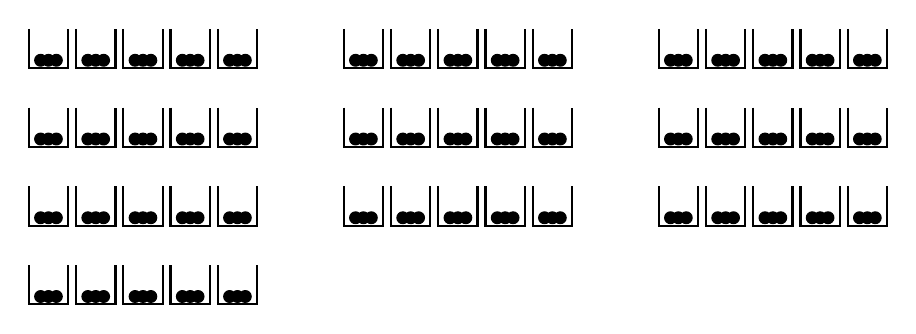
\begin{tikzpicture}[scale=0.5]
\newcommand\lax[3]{
\path[draw,thick,-] (#1-0.5,#2+0.5) -- (#1-0.5,#2-0.5) --
                    (#1+0.5,#2-0.5) -- (#1+0.5,#2+0.5);
\ifthenelse{\equal{#3}{1}}{\draw[fill=black] (#1,#2-0.3) circle (0.15);}{}
\ifthenelse{\equal{#3}{2}}{\draw[fill=black] (#1-0.2,#2-0.3) circle (0.15);}{}
\ifthenelse{\equal{#3}{2}}{\draw[fill=black] (#1+0.2,#2-0.3) circle (0.15);}{}
}
\newcommand\laa[7]{
    \lax{#1}{#2}{#3}
    \lax{#1+1.2}{#2}{#4}
    \lax{#1+2.4}{#2}{#5}
    \lax{#1+3.6}{#2}{#6}
    \lax{#1+4.8}{#2}{#7}
}

\laa{0}{0}{1}{1}{0}{0}{0}
\laa{0}{-2}{1}{0}{1}{0}{0}
\laa{0}{-4}{1}{0}{0}{1}{0}
\laa{0}{-6}{1}{0}{0}{0}{1}
\laa{8}{0}{0}{1}{1}{0}{0}
\laa{8}{-2}{0}{1}{0}{1}{0}
\laa{8}{-4}{0}{1}{0}{0}{1}
\laa{16}{0}{0}{0}{1}{1}{0}
\laa{16}{-2}{0}{0}{1}{0}{1}
\laa{16}{-4}{0}{0}{0}{1}{1}

\end{tikzpicture}
\end{center}

在这种情形下，答案就是二项式系数 ${n \choose k}$。

\textit{情形二}：一个盒子可以放多个球。例如，当 $n=5$、$k=2$ 时，共有 15 种方案：

\begin{center}
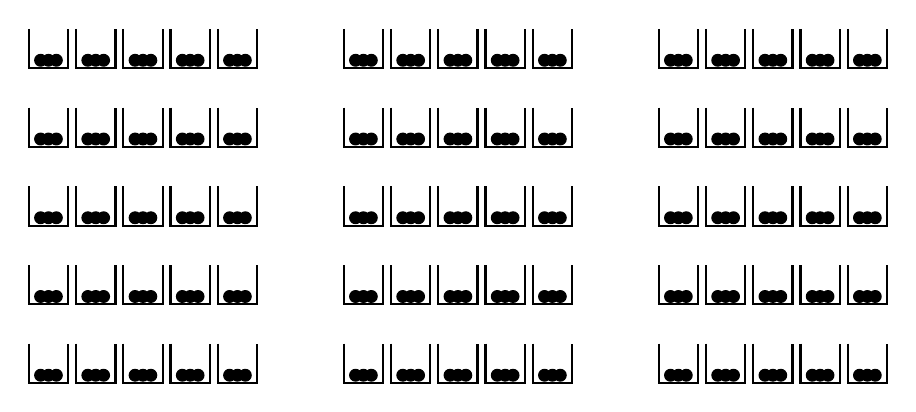
\begin{tikzpicture}[scale=0.5]
\newcommand\lax[3]{
\path[draw,thick,-] (#1-0.5,#2+0.5) -- (#1-0.5,#2-0.5) --
                    (#1+0.5,#2-0.5) -- (#1+0.5,#2+0.5);
\ifthenelse{\equal{#3}{1}}{\draw[fill=black] (#1,#2-0.3) circle (0.15);}{}
\ifthenelse{\equal{#3}{2}}{\draw[fill=black] (#1-0.2,#2-0.3) circle (0.15);}{}
\ifthenelse{\equal{#3}{2}}{\draw[fill=black] (#1+0.2,#2-0.3) circle (0.15);}{}
}
\newcommand\laa[7]{
    \lax{#1}{#2}{#3}
    \lax{#1+1.2}{#2}{#4}
    \lax{#1+2.4}{#2}{#5}
    \lax{#1+3.6}{#2}{#6}
    \lax{#1+4.8}{#2}{#7}
}

\laa{0}{0}{2}{0}{0}{0}{0}
\laa{0}{-2}{1}{1}{0}{0}{0}
\laa{0}{-4}{1}{0}{1}{0}{0}
\laa{0}{-6}{1}{0}{0}{1}{0}
\laa{0}{-8}{1}{0}{0}{0}{1}
\laa{8}{0}{0}{2}{0}{0}{0}
\laa{8}{-2}{0}{1}{1}{0}{0}
\laa{8}{-4}{0}{1}{0}{1}{0}
\laa{8}{-6}{0}{1}{0}{0}{1}
\laa{8}{-8}{0}{0}{2}{0}{0}
\laa{16}{0}{0}{0}{1}{1}{0}
\laa{16}{-2}{0}{0}{1}{0}{1}
\laa{16}{-4}{0}{0}{0}{2}{0}
\laa{16}{-6}{0}{0}{0}{1}{1}
\laa{16}{-8}{0}{0}{0}{0}{2}

\end{tikzpicture}
\end{center}

把球放入盒子的过程可以表示为由符号“o”和“$\rightarrow$”组成的字符串。初始时位于最左侧盒子；“o”表示在当前盒子中放一个球，“$\rightarrow$”表示向右移动到下一个盒子。

采用这种表示，每种方案对应一个含 $k$ 个“o”和 $n-1$ 个“$\rightarrow$”的字符串。例如，上图右上角的方案对应字符串“$\rightarrow$ $\rightarrow$ o $\rightarrow$ o $\rightarrow$”。因此，方案数为 ${k+n-1 \choose k}$。

\textit{情形三}：每个盒子至多放一个球，并且任意两个相邻盒子不能同时有球。例如，当 $n=5$、$k=2$ 时，共有 6 种方案：


\begin{center}
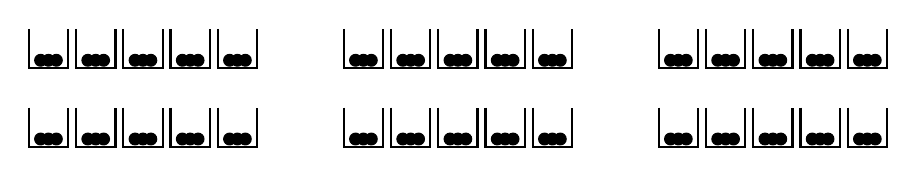
\begin{tikzpicture}[scale=0.5]
\newcommand\lax[3]{
\path[draw,thick,-] (#1-0.5,#2+0.5) -- (#1-0.5,#2-0.5) --
                    (#1+0.5,#2-0.5) -- (#1+0.5,#2+0.5);
\ifthenelse{\equal{#3}{1}}{\draw[fill=black] (#1,#2-0.3) circle (0.15);}{}
\ifthenelse{\equal{#3}{2}}{\draw[fill=black] (#1-0.2,#2-0.3) circle (0.15);}{}
\ifthenelse{\equal{#3}{2}}{\draw[fill=black] (#1+0.2,#2-0.3) circle (0.15);}{}
}
\newcommand\laa[7]{
    \lax{#1}{#2}{#3}
    \lax{#1+1.2}{#2}{#4}
    \lax{#1+2.4}{#2}{#5}
    \lax{#1+3.6}{#2}{#6}
    \lax{#1+4.8}{#2}{#7}
}

\laa{0}{0}{1}{0}{1}{0}{0}
\laa{0}{-2}{1}{0}{0}{1}{0}
\laa{8}{0}{1}{0}{0}{0}{1}
\laa{8}{-2}{0}{1}{0}{1}{0}
\laa{16}{0}{0}{1}{0}{0}{1}
\laa{16}{-2}{0}{0}{1}{0}{1}
\end{tikzpicture}
\end{center}

在这种情形下，可以先放置 $k$ 个球，并在每两个相邻的有球盒子之间预留一个空盒子。余下任务是为剩余空盒子选择位置。这样的空盒子有 $n-2k+1$ 个，可放置的位置有 $k+1$ 个。因此，利用情形二的公式，方案数为 ${n-k+1 \choose n-2k+1}$。

\subsubsection{多项式系数}

\index{multinomial coefficient}

\key{多项式系数}
\[ {n \choose k_1,k_2,\ldots,k_m} = \frac{n!}{k_1! k_2! \cdots k_m!}, \]
表示把 $n$ 个元素划分成大小分别为 $k_1,k_2,\ldots,k_m$ 的子集的方法数，其中 $k_1+k_2+\cdots+k_m=n$。多项式系数可以看作二项式系数的推广；当 $m=2$ 时，上式就是二项式系数公式。

\section{Catalan 数}

\index{Catalan number}

\key{Catalan 数}
%\footnote{E. C. Catalan (1814--1894) was a Belgian mathematician.}
$C_n$ 等于由 $n$ 个左括号和 $n$ 个右括号组成的合法括号序列数量。

例如，$C_3=5$，因为用三个左括号和三个右括号可以构造以下括号序列：

\begin{itemize}[noitemsep]
\item \texttt{()()()}
\item \texttt{(())()}
\item \texttt{()(())}
\item \texttt{((()))}
\item \texttt{(()())}
\end{itemize}

\subsubsection{括号序列}

\index{parenthesis expression}

什么是\emph{合法括号序列}？以下规则精确定义了所有合法括号序列：

\begin{itemize}
\item 空括号序列合法。
\item 若序列 $A$ 合法，则序列 \texttt{(}$A$\texttt{)} 也合法。
\item 若序列 $A$、$B$ 合法，则序列 $AB$ 也合法。
\end{itemize}

合法括号序列还有另一种刻画：它的任意前缀中，左括号数量都不少于右括号数量；并且完整序列中左右括号数量相等。

\subsubsection{公式一}

Catalan 数可以用公式
\[ C_n = \sum_{i=0}^{n-1} C_{i} C_{n-i-1}.\]

计算。求和枚举把序列分成两个合法部分的方法，其中第一部分非空且尽可能短。对于每个 $i$，第一部分包含 $i+1$ 对括号，序列数量是以下两项的乘积：

\begin{itemize}
\item $C_i$：使用第一部分除最外层括号之外的括号构造序列的方法数；
\item $C_{n-i-1}$：使用第二部分的括号构造序列的方法数。
\end{itemize}

边界条件为 $C_0=1$，因为用零对括号可以构造一个空括号序列。

\subsubsection{公式二}

Catalan 数也可以用二项式系数计算：
\[ C_n = \frac{1}{n+1} {2n \choose n}\]
该公式可解释如下。

由 $n$ 个左括号和 $n$ 个右括号构成的括号序列（不要求合法）共有 ${2n \choose n}$ 个。下面计算其中\emph{不合法}序列的数量。

如果括号序列不合法，它必有一个前缀，其中右括号数量超过左括号数量。把这样一个最短前缀中的每个括号反转。例如，序列 \texttt{())()(} 含有前缀 \texttt{())}，反转该前缀后得到 \texttt{)((()(}。

所得序列包含 $n+1$ 个左括号和 $n-1$ 个右括号。这类序列有 ${2n \choose n+1}$ 个，恰好等于不合法括号序列的数量。因此，合法括号序列数为
\[{2n \choose n}-{2n \choose n+1} = {2n \choose n} - \frac{n}{n+1} {2n \choose n} = \frac{1}{n+1} {2n \choose n}.\]

\subsubsection{树的计数}

Catalan 数还与树有关：

\begin{itemize}
\item 含 $n$ 个结点的二叉树有 $C_n$ 棵；
\item 含 $n$ 个结点的有根树有 $C_{n-1}$ 棵。
\end{itemize}
\noindent
例如，由 $C_3=5$ 可知，对应的二叉树为

\begin{center}
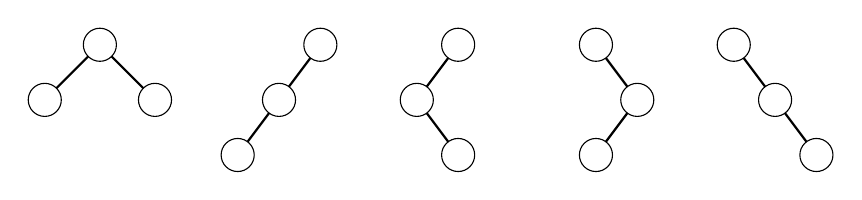
\begin{tikzpicture}[scale=0.7]
\path[draw,thick,-] (0,0) -- (-1,-1);
\path[draw,thick,-] (0,0) -- (1,-1);
\draw[fill=white] (0,0) circle (0.3);
\draw[fill=white] (-1,-1) circle (0.3);
\draw[fill=white] (1,-1) circle (0.3);

\path[draw,thick,-] (4,0) -- (4-0.75,-1) -- (4-1.5,-2);
\draw[fill=white] (4,0) circle (0.3);
\draw[fill=white] (4-0.75,-1) circle (0.3);
\draw[fill=white] (4-1.5,-2) circle (0.3);

\path[draw,thick,-] (6.5,0) -- (6.5-0.75,-1) -- (6.5-0,-2);
\draw[fill=white] (6.5,0) circle (0.3);
\draw[fill=white] (6.5-0.75,-1) circle (0.3);
\draw[fill=white] (6.5-0,-2) circle (0.3);

\path[draw,thick,-] (9,0) -- (9+0.75,-1) -- (9-0,-2);
\draw[fill=white] (9,0) circle (0.3);
\draw[fill=white] (9+0.75,-1) circle (0.3);
\draw[fill=white] (9-0,-2) circle (0.3);

\path[draw,thick,-] (11.5,0) -- (11.5+0.75,-1) -- (11.5+1.5,-2);
\draw[fill=white] (11.5,0) circle (0.3);
\draw[fill=white] (11.5+0.75,-1) circle (0.3);
\draw[fill=white] (11.5+1.5,-2) circle (0.3);
\end{tikzpicture}
\end{center}
而对应的有根树为
\begin{center}
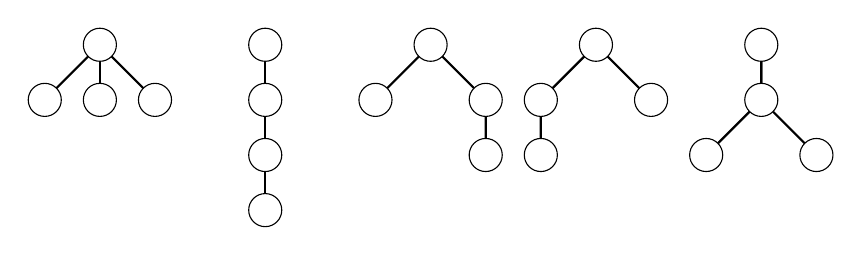
\begin{tikzpicture}[scale=0.7]
\path[draw,thick,-] (0,0) -- (-1,-1);
\path[draw,thick,-] (0,0) -- (0,-1);
\path[draw,thick,-] (0,0) -- (1,-1);
\draw[fill=white] (0,0) circle (0.3);
\draw[fill=white] (-1,-1) circle (0.3);
\draw[fill=white] (0,-1) circle (0.3);
\draw[fill=white] (1,-1) circle (0.3);

\path[draw,thick,-] (3,0) -- (3,-1) -- (3,-2) -- (3,-3);
\draw[fill=white] (3,0) circle (0.3);
\draw[fill=white] (3,-1) circle (0.3);
\draw[fill=white] (3,-2) circle (0.3);
\draw[fill=white] (3,-3) circle (0.3);

\path[draw,thick,-] (6+0,0) -- (6-1,-1);
\path[draw,thick,-] (6+0,0) -- (6+1,-1) -- (6+1,-2);
\draw[fill=white] (6+0,0) circle (0.3);
\draw[fill=white] (6-1,-1) circle (0.3);
\draw[fill=white] (6+1,-1) circle (0.3);
\draw[fill=white] (6+1,-2) circle (0.3);

\path[draw,thick,-] (9+0,0) -- (9+1,-1);
\path[draw,thick,-] (9+0,0) -- (9-1,-1) -- (9-1,-2);
\draw[fill=white] (9+0,0) circle (0.3);
\draw[fill=white] (9+1,-1) circle (0.3);
\draw[fill=white] (9-1,-1) circle (0.3);
\draw[fill=white] (9-1,-2) circle (0.3);

\path[draw,thick,-] (12+0,0) -- (12+0,-1) -- (12-1,-2);
\path[draw,thick,-] (12+0,0) -- (12+0,-1) -- (12+1,-2);
\draw[fill=white] (12+0,0) circle (0.3);
\draw[fill=white] (12+0,-1) circle (0.3);
\draw[fill=white] (12-1,-2) circle (0.3);
\draw[fill=white] (12+1,-2) circle (0.3);

\end{tikzpicture}
\end{center}

\section{容斥原理}

\index{inclusion-exclusion}

\key{容斥原理}是一种计数技术，可以在已知各交集大小时计算集合并集的大小，也可以反过来计算。一个简单例子是公式
\[ |A \cup B| = |A| + |B| - |A \cap B|,\]
其中 $A$、$B$ 为集合，$|X|$ 表示 $X$ 的大小。该公式可用下图说明：

\begin{center}
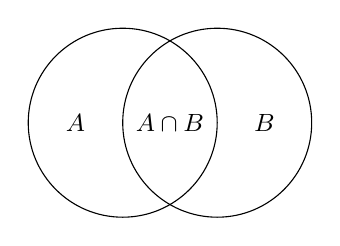
\begin{tikzpicture}[scale=0.8]

\draw (0,0) circle (1.5);
\draw (1.5,0) circle (1.5);

\node at (-0.75,0) {\small $A$};
\node at (2.25,0) {\small $B$};
\node at (0.75,0) {\small $A \cap B$};

\end{tikzpicture}
\end{center}

目标是计算并集 $A \cup B$ 的大小，它对应至少属于一个圆的区域面积。由图可见，可以先把 $A$ 与 $B$ 的面积相加，再减去 $A \cap B$ 的面积，从而得到 $A \cup B$ 的面积。

同样的思想也适用于更多集合。当有三个集合时，容斥公式为
\[ |A \cup B \cup C| = |A| + |B| + |C| - |A \cap B|  - |A \cap C|  - |B \cap C| + |A \cap B \cap C| \]
对应图示为

\begin{center}
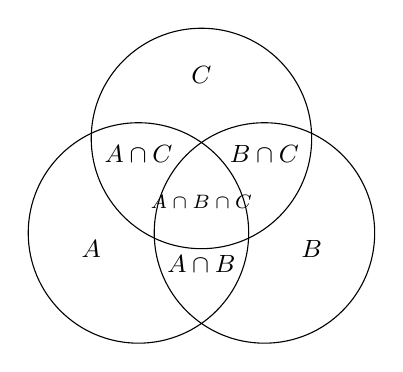
\begin{tikzpicture}[scale=0.8]

\draw (0,0) circle (1.75);
\draw (2,0) circle (1.75);
\draw (1,1.5) circle (1.75);

\node at (-0.75,-0.25) {\small $A$};
\node at (2.75,-0.25) {\small $B$};
\node at (1,2.5) {\small $C$};
\node at (1,-0.5) {\small $A \cap B$};
\node at (0,1.25) {\small $A \cap C$};
\node at (2,1.25) {\small $B \cap C$};
\node at (1,0.5) {\scriptsize $A \cap B \cap C$};

\end{tikzpicture}
\end{center}

一般情况下，可以枚举由 $X_1,X_2,\ldots,X_n$ 中若干集合组成的所有交集，计算并集 $X_1 \cup X_2 \cup \cdots \cup X_n$ 的大小。若交集包含奇数个集合，就把它的大小加到答案中；否则从答案中减去。

反过来，也有根据并集大小计算交集大小的类似公式。例如，
\[ |A \cap B| = |A| + |B| - |A \cup B|\]
and
\[ |A \cap B \cap C| = |A| + |B| + |C| - |A \cup B|  - |A \cup C|  - |B \cup C| + |A \cup B \cup C| .\]

\subsubsection{错排}

\index{derangement}

例如，计算元素 $\{1,2,\ldots,n\}$ 的\key{错排}数量，即没有任何元素留在原位置的排列数。当 $n=3$ 时，共有两个错排：$(2,3,1)$ 和 $(3,1,2)$。

一种解法是使用容斥原理。令 $X_k$ 为第 $k$ 个位置恰好放置元素 $k$ 的排列集合。当 $n=3$ 时，各集合如下：
\[
\begin{array}{lcl}
X_1 & = & \{(1,2,3),(1,3,2)\} \\
X_2 & = & \{(1,2,3),(3,2,1)\} \\
X_3 & = & \{(1,2,3),(2,1,3)\} \\
\end{array}
\]
利用这些集合，错排数等于
\[ n! - |X_1 \cup X_2 \cup \cdots \cup X_n|, \]
因此只需计算并集大小。利用容斥原理，可将其归约为高效计算各交集大小。当 $n=3$ 时，$|X_1 \cup X_2 \cup X_3|$ 为
\[
\begin{array}{lcl}
 & & |X_1| + |X_2| + |X_3| - |X_1 \cap X_2|  - |X_1 \cap X_3|  - |X_2 \cap X_3| + |X_1 \cap X_2 \cap X_3| \\
 & = & 2+2+2-1-1-1+1 \\
 & = & 4, \\
\end{array}
\]
所以错排数为 $3!-4=2$。

这个问题也可以不用容斥原理求解。令 $f(n)$ 表示 $\{1,2,\ldots,n\}$ 的错排数，可以使用递推式：

\begin{equation*}
    f(n) = \begin{cases}
               0               & n = 1\\
               1               & n = 2\\
               (n-1)(f(n-2) + f(n-1)) & n>2 \\
           \end{cases}
\end{equation*}

推导该公式时，考虑错排中元素 1 被如何替换。用于替换元素 1 的元素 $x$ 有 $n-1$ 种选择；对每种选择，又有两种情况：

\textit{情况一}：再用元素 1 替换元素 $x$。此后只需构造其余 $n-2$ 个元素的错排。

\textit{情况二}：用 1 以外的某个元素替换元素 $x$。此时需要构造 $n-1$ 个元素的错排，因为不能再用元素 1 替换元素 $x$，而所有其他元素仍必须改变位置。

\section{Burnside 引理}

\index{Burnside's lemma}

\key{Burnside 引理}
%\footnote{Actually, Burnside did not discover this lemma; he only mentioned it in his book \cite{bur97}.}
可用于计算组合数，并让每组相互对称的组合只计入一个代表。Burnside 引理指出，组合数量为
\[\sum_{k=1}^n \frac{c(k)}{n},\]
其中共有 $n$ 种改变组合位置的方式，应用第 $k$ 种方式后保持不变的组合有 $c(k)$ 个。

例如，计算由 $n$ 颗珠子组成的项链数量，每颗珠子有 $m$ 种可选颜色。如果两条项链旋转后相同，就认为它们对称。例如，项链
\begin{center}
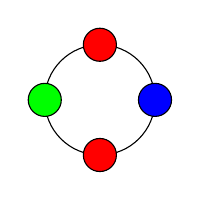
\begin{tikzpicture}[scale=0.7]
\draw[fill=white] (0,0) circle (1);
\draw[fill=red] (0,1) circle (0.3);
\draw[fill=blue] (1,0) circle (0.3);
\draw[fill=red] (0,-1) circle (0.3);
\draw[fill=green] (-1,0) circle (0.3);
\end{tikzpicture}
\end{center}
有以下与之对称的项链：
\begin{center}
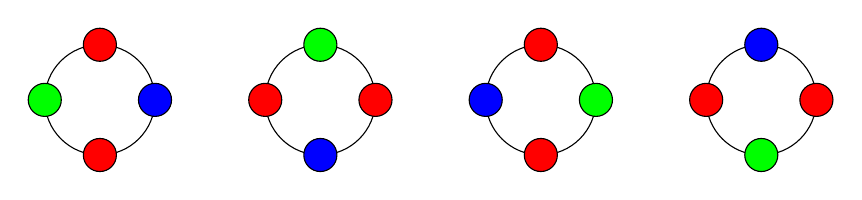
\begin{tikzpicture}[scale=0.7]
\draw[fill=white] (0,0) circle (1);
\draw[fill=red] (0,1) circle (0.3);
\draw[fill=blue] (1,0) circle (0.3);
\draw[fill=red] (0,-1) circle (0.3);
\draw[fill=green] (-1,0) circle (0.3);

\draw[fill=white] (4,0) circle (1);
\draw[fill=green] (4+0,1) circle (0.3);
\draw[fill=red] (4+1,0) circle (0.3);
\draw[fill=blue] (4+0,-1) circle (0.3);
\draw[fill=red] (4+-1,0) circle (0.3);

\draw[fill=white] (8,0) circle (1);
\draw[fill=red] (8+0,1) circle (0.3);
\draw[fill=green] (8+1,0) circle (0.3);
\draw[fill=red] (8+0,-1) circle (0.3);
\draw[fill=blue] (8+-1,0) circle (0.3);

\draw[fill=white] (12,0) circle (1);
\draw[fill=blue] (12+0,1) circle (0.3);
\draw[fill=red] (12+1,0) circle (0.3);
\draw[fill=green] (12+0,-1) circle (0.3);
\draw[fill=red] (12+-1,0) circle (0.3);
\end{tikzpicture}
\end{center}
一条项链的位置有 $n$ 种改变方式，因为可以顺时针旋转 $0,1,\ldots,n-1$ 步。旋转 0 步时，所有 $m^n$ 条项链都保持不变；旋转 1 步时，只有全部珠子颜色相同的 $m$ 条项链保持不变。

更一般地，旋转 $k$ 步时，共有
\[m^{\textrm{gcd}(k,n)}\]
条项链保持不变，其中 $\textrm{gcd}(k,n)$ 是 $k$ 与 $n$ 的最大公约数。原因是大小为 $\textrm{gcd}(k,n)$ 的珠子块会相互替换。因此，根据 Burnside 引理，项链数量为
\[\sum_{i=0}^{n-1} \frac{m^{\textrm{gcd}(i,n)}}{n}. \]
例如，用 3 种颜色构成长度为 4 的项链共有
\[\frac{3^4+3+3^2+3}{4} = 24. \]

\section{Cayley 公式}

\index{Cayley's formula}

\key{Cayley 公式}
% \footnote{While the formula is named after A. Cayley,
% who studied it in 1889, it was discovered earlier by C. W. Borchardt in 1860.}
指出，含有 $n$ 个结点的有标号树共有 $n^{n-2}$ 棵。结点编号为 $1,2,\ldots,n$；只要两棵树的结构或标号不同，就视为不同的树。

\begin{samepage}
例如，当 $n=4$ 时，有标号树共有 $4^{4-2}=16$ 棵：

\begin{center}
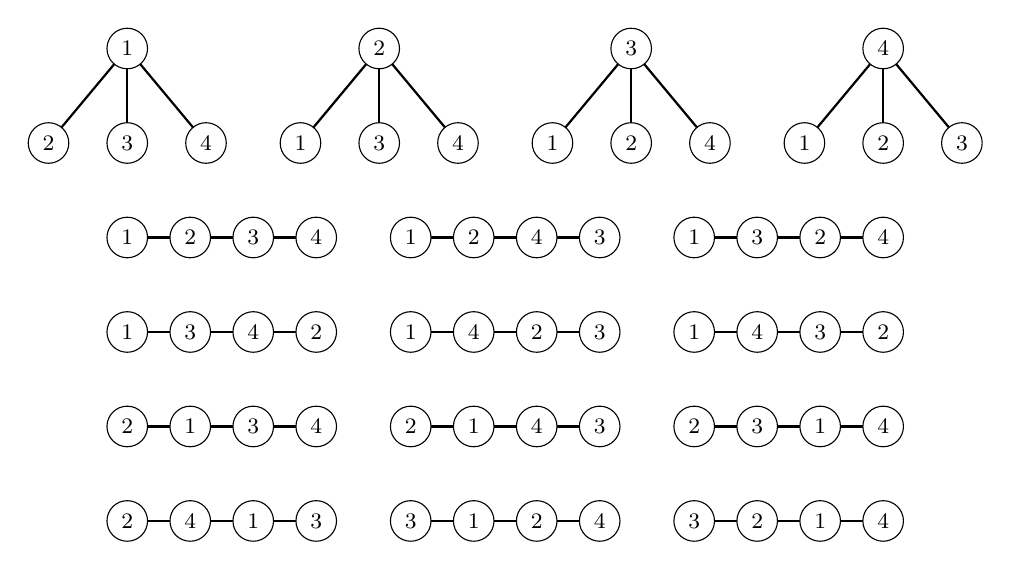
\begin{tikzpicture}[scale=0.8]
\footnotesize

\newcommand\puua[6]{
\path[draw,thick,-] (#1,#2) -- (#1-1.25,#2-1.5);
\path[draw,thick,-] (#1,#2) -- (#1,#2-1.5);
\path[draw,thick,-] (#1,#2) -- (#1+1.25,#2-1.5);
\node[draw, circle, fill=white] at (#1,#2) {#3};
\node[draw, circle, fill=white] at (#1-1.25,#2-1.5) {#4};
\node[draw, circle, fill=white] at (#1,#2-1.5) {#5};
\node[draw, circle, fill=white] at (#1+1.25,#2-1.5) {#6};
}
\newcommand\puub[6]{
\path[draw,thick,-] (#1,#2) -- (#1+1,#2);
\path[draw,thick,-] (#1+1,#2) -- (#1+2,#2);
\path[draw,thick,-] (#1+2,#2) -- (#1+3,#2);
\node[draw, circle, fill=white] at (#1,#2) {#3};
\node[draw, circle, fill=white] at (#1+1,#2) {#4};
\node[draw, circle, fill=white] at (#1+2,#2) {#5};
\node[draw, circle, fill=white] at (#1+3,#2) {#6};
}

\puua{0}{0}{1}{2}{3}{4}
\puua{4}{0}{2}{1}{3}{4}
\puua{8}{0}{3}{1}{2}{4}
\puua{12}{0}{4}{1}{2}{3}

\puub{0}{-3}{1}{2}{3}{4}
\puub{4.5}{-3}{1}{2}{4}{3}
\puub{9}{-3}{1}{3}{2}{4}
\puub{0}{-4.5}{1}{3}{4}{2}
\puub{4.5}{-4.5}{1}{4}{2}{3}
\puub{9}{-4.5}{1}{4}{3}{2}
\puub{0}{-6}{2}{1}{3}{4}
\puub{4.5}{-6}{2}{1}{4}{3}
\puub{9}{-6}{2}{3}{1}{4}
\puub{0}{-7.5}{2}{4}{1}{3}
\puub{4.5}{-7.5}{3}{1}{2}{4}
\puub{9}{-7.5}{3}{2}{1}{4}
\end{tikzpicture}
\end{center}
\end{samepage}

下面说明如何用 Prüfer 编码推导 Cayley 公式。

\subsubsection{Prüfer 编码}

\index{Prüfer code}

\key{Prüfer 编码}
%\footnote{In 1918, H. Prüfer proved Cayley's theorem using Prüfer codes \cite{pru18}.}
是由 $n-2$ 个数构成、用于描述一棵有标号树的序列。构造编码时，要从树中依次删除 $n-2$ 个叶结点。每一步删除标号最小的叶结点，并把它唯一邻居的标号加入编码。

例如，计算下图的 Prüfer 编码：
\begin{center}
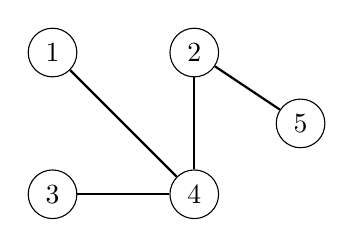
\begin{tikzpicture}[scale=0.9]
\node[draw, circle] (1) at (2,3) {$1$};
\node[draw, circle] (2) at (4,3) {$2$};
\node[draw, circle] (3) at (2,1) {$3$};
\node[draw, circle] (4) at (4,1) {$4$};
\node[draw, circle] (5) at (5.5,2) {$5$};

\path[draw,thick,-] (1) -- (4);
\path[draw,thick,-] (3) -- (4);
\path[draw,thick,-] (2) -- (4);
\path[draw,thick,-] (2) -- (5);
\end{tikzpicture}
\end{center}

首先删除结点 1，并把结点 4 加入编码：
\begin{center}
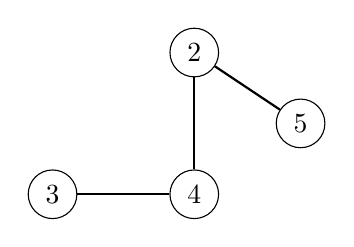
\begin{tikzpicture}[scale=0.9]
%\node[draw, circle] (1) at (2,3) {$1$};
\node[draw, circle] (2) at (4,3) {$2$};
\node[draw, circle] (3) at (2,1) {$3$};
\node[draw, circle] (4) at (4,1) {$4$};
\node[draw, circle] (5) at (5.5,2) {$5$};

%\path[draw,thick,-] (1) -- (4);
\path[draw,thick,-] (3) -- (4);
\path[draw,thick,-] (2) -- (4);
\path[draw,thick,-] (2) -- (5);
\end{tikzpicture}
\end{center}

然后删除结点 3，并把结点 4 加入编码：
\begin{center}
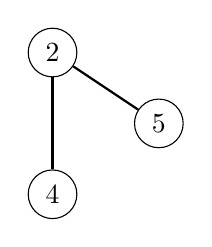
\begin{tikzpicture}[scale=0.9]
%\node[draw, circle] (1) at (2,3) {$1$};
\node[draw, circle] (2) at (4,3) {$2$};
%\node[draw, circle] (3) at (2,1) {$3$};
\node[draw, circle] (4) at (4,1) {$4$};
\node[draw, circle] (5) at (5.5,2) {$5$};

%\path[draw,thick,-] (1) -- (4);
%\path[draw,thick,-] (3) -- (4);
\path[draw,thick,-] (2) -- (4);
\path[draw,thick,-] (2) -- (5);
\end{tikzpicture}
\end{center}

最后删除结点 4，并把结点 2 加入编码：
\begin{center}
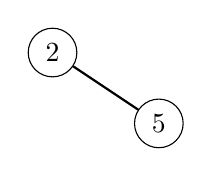
\begin{tikzpicture}[scale=0.9]
%\node[draw, circle] (1) at (2,3) {$1$};
\node[draw, circle] (2) at (4,3) {$2$};
%\node[draw, circle] (3) at (2,1) {$3$};
%\node[draw, circle] (4) at (4,1) {$4$};
\node[draw, circle] (5) at (5.5,2) {$5$};

%\path[draw,thick,-] (1) -- (4);
%\path[draw,thick,-] (3) -- (4);
%\path[draw,thick,-] (2) -- (4);
\path[draw,thick,-] (2) -- (5);
\end{tikzpicture}
\end{center}

因此，该图的 Prüfer 编码为 $[4,4,2]$。

任意树都能构造 Prüfer 编码；更重要的是，也能从 Prüfer 编码恢复原树。因此，含 $n$ 个结点的有标号树数量等于长度为 $n-2$、每项取值为 $1\ldots n$ 的 Prüfer 编码数量，即 $n^{n-2}$。
